
\section{Auditory-nerve fibres}\label{sec:an}

The data are the public recordings of single auditory-nerve fibres of the gerbil by Heeringa and colleagues~\cite{Heeringa2024}.
Two of their protocols serve our questions, and each test uses the recordings of one protocol. In rate-level recordings, tones at the
best frequency, the frequency the fibre responds to most, are played at up to 27 sound levels with 10 presentations each; these serve
the test of shape. Phase-locking recordings were made in fibres with best frequencies below about 5~kHz, where spikes lock to the phase
of the tone. In them, tones are played at 5 to 8 sound levels with 20 to 40 presentations each; the larger number of presentations serves the
test of discreteness, which compares the mean counts of neighbouring sound levels. Counts are taken in a window of 50~ms from tone onset.
Every test below was fixed, with its decision rule and its controls on synthetic fibres, before the data were analysed;
Section~\ref{sec:methods} gives the details. Table~\ref{tab:an} lists the tests and whether their registered rule held.

\begin{table}[tp]
\caption{Registered tests on auditory-nerve fibres. $d$: log-likelihood of the predicted shape minus that of the symmetric sigmoid,
in nats per fibre; LB: bootstrap 95\% lower bound of the mean of $d$; $\sigma$: spread of the level distribution implied by the fitted
shape; $D$: number of significantly different mean counts across the tested sound levels; $K$: number of steps of the optimal
staircase at the fibre's peak and spontaneous counts, for the count model named in the row; drift: a slow change of rate across
presentations; Fano factor: variance of the count divided by its mean. The fibres of the two age groups are 881 of the 950; the other 69 come from
middle-aged animals and were not part of the registered replication.}\label{tab:an}
\centering
\small
\begin{tabular}{>{\raggedright\arraybackslash}p{3.4cm}r>{\raggedright\arraybackslash}p{4.4cm}>{\raggedright\arraybackslash}p{3.6cm}}
\hline
test & fibres & registered rule & result\\
\hline
shape (bell-shaped level law) & 950 & LB $>0$ and median $\sigma$ in $[6,20]$ dB & LB $0.1495$, $\sigma$ $8.53$ dB: held\\
shape, young-adult animals & 608 & LB $>0$ & LB $0.1427$: held\\
shape, quiet-aged animals & 273 & LB $>0$ & LB $0.0768$: held\\
exact square-root shape against the registered shape & 950 & LB of the mean log-likelihood gain $>0$ & LB $-0.1062$: did not hold\\
shape against the curve of opposite asymmetry & 950 & LB of the mean log-likelihood gain $>0$ & LB $1.1048$: held\\
staircase, Poisson counts, 50 ms & 265 & $D\le K$ in at least $80\%$ of fibres & $51.7\%$: did not hold\\
drift explains the excess & 265 & drift in at least $30\%$ of fibres & $5.7\%$: did not hold\\
staircase, Poisson counts, 75 ms & 271 & $D\le K$ in at least $80\%$ of fibres & $55.7\%$: did not hold\\
counts as variable as Poisson counts & 265 & median Fano factor in $[0.8,1.2]$ & median $0.355$: did not hold\\
staircase, binomial counts, 50 ms & 265 & $D\le K$ in at least $80\%$ of fibres & $88.3\%$: held\\
staircase, counts matched to each fibre's Fano factor, 50 ms & 265 & $D\le K$ in at least $80\%$ of fibres & $82.3\%$: held\\
staircase, counts matched to each fibre's Fano factor at every rate, 50 ms & 265 & $D\le K$ in at least $80\%$ of fibres & $77.0\%$: did not hold\\
staircase, likelihood statistic, count matched at every rate, 50 ms & 265 & at least $80\%$ of fibres consistent with at most $K$ steps & $40.4\%$: did not hold\\
the same, with the range from the spontaneous count & 265 & the same & $49.4\%$: did not hold\\
\hline
\end{tabular}
\end{table}

\emph{Shape.} The decibel amplitude of natural sounds has a roughly symmetric bell-shaped distribution~\cite{Escabi2003}. Take the
distribution of sound level $L$ to be Gaussian with mean $\mu$ and spread $\sigma$, so that $F_S(L)=\Phi((L-\mu)/\sigma)$, where $\Phi$
is the standard normal distribution function. For a small spontaneous count $r_0$, the fitted value of $\lambda$, the large-$A$ form of Section~\ref{sec:laughlin}
becomes $r_0+A\,\Phi((L-\mu)/\sigma)^2$, an asymmetric sigmoid in $L$. The square of the S-shaped $\Phi$ rises from its floor more steeply than it
approaches its ceiling, unlike a symmetric sigmoid (Fig~\ref{fig:rlf}A). This is the form the test registered. We compared this predicted
shape with the symmetric sigmoid, the usual description of rate-level functions, which has the same four parameters (spontaneous count, peak count, centre and width),
by Poisson likelihood on the single-trial counts of 950 fibres. A single fibre at ten presentations distinguishes the two shapes only
weakly, so the decision pooled the fibres. For each fibre, $d$ is the log-likelihood of the predicted shape minus that of the sigmoid, in nats over all its
single-trial counts. The mean of $d$ over fibres was $0.2027$, with a bootstrap lower bound of $0.1495$. Only $50.8\%$ of fibres favour the predicted shape individually, so the pooled preference comes
from a minority of fibres with a large difference (Fig~\ref{fig:rlf}B). The decision rule asked for a positive pooled mean and
a median spread $\sigma$ between 6 and 20~dB, not for a majority of fibres. Fibres of one animal need not be independent; a
bootstrap that draws the 103 animals with all their fibres, a reading made after the test, gives a lower bound of $0.1466$. In a split made after the test, the preference was strongest in fibres with large peak counts and in fibres with a low
spontaneous count (below 0.5 per window), $78.9\%$ of which favoured the predicted shape. It held separately in young-adult and in quiet-aged animals, aged animals raised in a quiet
environment so that noise damage to the cochlea is kept small~\cite{Heeringa2024}, with lower bounds of $0.1427$ and $0.0768$. The
spread $\sigma$ that the fitted shapes imply for the level distribution has a median of $8.53$~dB. From recordings of natural sounds,
Escab\'i and colleagues measured standard deviations of the decibel amplitude in frequency bands of $9.1$~dB for environmental
sounds, $13.3$~dB for vocalizations and $14.8$~dB for speech, so the fitted spread lies just below the range of natural sounds.

Section~\ref{sec:laughlin} also gives the exact form for any spontaneous count,
$\bigl(\sqrt{r_0}+(\sqrt{r_0+A}-\sqrt{r_0})\,\Phi\bigr)^2$. In the registered form the spontaneous count is added to the
stimulus-driven count; in the exact form the two mix inside the square. The prediction of the exact form failed: a second registered test found that it describes
the fibres worse than the registered one, with a mean log-likelihood difference of $-0.0904$ per fibre and a bootstrap lower bound of
$-0.1062$, although it still beats the symmetric sigmoid. The fibres therefore behave as if their spontaneous count were an offset
added to the stimulus-driven count.
A third registered test compared the predicted form with the complementary log-log curve $r_0+A(1-e^{-e^{(L-\mu)/\sigma_{\rm s}}})$,
which has four parameters and the opposite direction of asymmetry. The predicted form fitted better: the mean of $d$ was $1.2463$,
with a bootstrap lower bound of $1.1048$, and $80.2\%$ of fibres favoured it. Against the Gompertz curve
$r_0+A\,e^{-e^{-(L-\mu)/\sigma_{\rm s}}}$, whose asymmetry has the predicted direction and is stronger, the predicted form fitted
worse, with a mean difference of $-0.1834$ and a lower bound of $-0.2432$; this comparison is a reading, not a registered rule. The
fibres thus show the predicted direction of asymmetry, while the predicted form is not the best curve of that direction. Fig~\ref{fig:rlf}A shows a fibre
chosen by a rule fixed before plotting: among the 50 fibres whose fitted peak count is closest to the median, the one whose difference
$d$ is the median.

\begin{figure}[!ht]
\centering
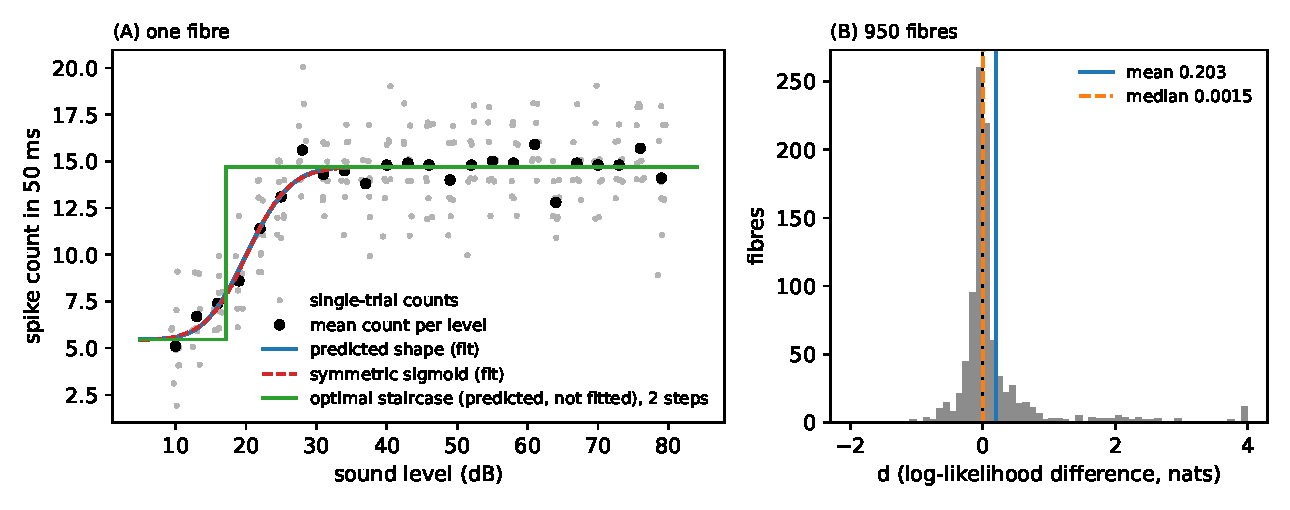
\includegraphics[width=\textwidth]{figs/fig_rlf.pdf}
\caption{\textbf{The rate-level functions and the predicted shape.} (A) One fibre, chosen by a rule fixed before any plot was made:
among the 50 fibres whose fitted peak count is closest to the median over all fibres, the one with the median $d$. Grey points: single-trial
counts in 50~ms; black points: mean count per sound level; solid line: fitted predicted shape; dashed line: fitted symmetric sigmoid;
step line: the staircase of Proposition~\ref{prop:L1}, predicted and not fitted, for a Gaussian level law with the fitted mean and
spread, at the fibre's fitted spontaneous count $5.46$ and peak count $9.25$ above it, where the capacity-achieving input has two
rates. The staircase is what an optimal fibre with these counts would show; the data are compared with it through the number of
distinct mean counts, not point by point, and Fig~\ref{fig:dk}C shows that comparison for one fibre of the discreteness test. For this fibre the two fitted shapes nearly coincide ($d=-0.035$). (B) The difference $d$
for all 950 fibres, with zero, the mean $0.203$ and the median $0.0015$ marked; the median near zero shows that the pooled advantage
comes from a minority of fibres; one value below $-2$ and ten above $4$ are drawn at the ends.}\label{fig:rlf}
\end{figure}

\emph{Discreteness.} Proposition~\ref{prop:L1} predicts that an optimal fibre shows at most $K$ different mean counts across any set of
sound levels, where $K$ is the number of steps of the optimal staircase at the fibre's peak and spontaneous counts. Measured
mean counts are noisy, so two neighbouring sound levels count as having different mean counts only when a test finds their counts
significantly different. We counted the different mean counts $D$ in this way, with an exact binomial test between neighbouring levels
and Holm's correction for multiple comparisons~\cite{Holm1979} within each fibre (Section~\ref{sec:methods}). With $K$ computed for Poisson counts,
the bound $D\le K$ held in $51.7\%$ of the 265 fibres that met the selection rule of Section~\ref{sec:methods}, against the
registered $80\%$. Most excesses were of one rate: the difference
$D-K$ was $-1$ in 34 fibres, $0$ in 103, $+1$ in 103 ($38.9\%$), $+2$ in 23 and $+3$ in 2. A fully graded fibre would show as many distinct mean counts as tested sound
levels; only $8.7\%$ of fibres did, so the fibres are not fully graded either. Slow drift, a change of rate across the presentations
of one sound level, does not explain the excess: only $5.7\%$ of fibres drifted, close to the $4.5\%$ that the drift test marks in stationary synthetic fibres. Fibres with
an excess drifted no more often than the others. The recorded trials of most fibres end near 80~ms after tone onset, so 75~ms is the
longest window inside every trial; it raised the fraction only to $55.7\%$, with 271 fibres meeting the selection rule at that
window.

The counts, however, are not Poisson. The tests that follow were registered after the Poisson test had failed and in response to
it. Each had its rule and its bar of $80\%$ fixed before it was run (Section~\ref{sec:methods}). The Fano factor of a count, its variance across presentations divided by its mean, is 1 for
Poisson counts. Over the 1430 sound levels of the 265 fibres with a mean count of at least one, its median was $0.355$, with
quartiles $0.259$ and $0.524$, and $86.0\%$ of the levels lay below $0.67$. A count that varies less than a Poisson count has less
noise at each rate, so nearby rates are easier to tell apart, the optimal input of its counting channel can hold more rates, and the
$K$ above is too small for these fibres. The proof of Proposition~\ref{prop:L1} uses only that the count depends on the stimulus through the rate: for any counting
channel, the staircase built from a capacity-achieving input with finitely many mass points is an optimal tuning curve. We therefore
recomputed $K$ for a binomial count with $n$ trials and mean $r$, whose Fano factor is $1-r/n$. The binomial count is the simplest
count less variable than a Poisson one: a neuron that fires at most once in each of $n$ short bins of the window produces it. For a largest expected count $\lambda+A$ of 10 in the 50~ms window,
$n$ is 10 and each bin is 5~ms long, much longer than the absolute refractory period of about 0.6~ms of these fibres~\cite{Heeringa2024}.
The bins are a device of the model: the binomial count describes how regular the counts are, not the time course of recovery. Since the count takes only $n+1$
values, a capacity-achieving input with at most $n+1$ mass points exists~\cite{Favano2026}. For $n$ we took the smallest integer at
or above $\lambda+A$, the most regular binomial count that reaches the fibre's peak rate. With this $K$ the bound $D\le K$ held in
$88.3\%$ of the 265 fibres, above the registered $80\%$; five fibres with a Fano factor of at least one kept Poisson counts. The binomial $K$
exceeded the Poisson one by one rate in 177 fibres and by two in 28. The binomial count models the regularity of the fibres without
being fitted to it: at the fibre's mean count it is more regular than the fibre in 158 fibres and less regular in 102. A second
registered test therefore matched the count to each fibre. It used a Conway-Maxwell-Poisson count~\cite{Shmueli2005}, whose dispersion is set by one
parameter $\zeta$: the value 1 gives Poisson counts, and larger values give less variable ones. For each fibre $\zeta$ was chosen so
that the Fano factor at the fibre's mean count equals the measured one. With this $K$ the bound held in $82.3\%$ of the fibres, again
above the registered $80\%$. For this count, too, the capacity-achieving input has finitely many mass points, as S1 Text proves, and
$K$ is the number of mass points of the numerical solution on a grid of 801 rates.

The matched count still has one exponent per fibre, so its Fano factor hardly changes with the rate. Within each fibre the measured
Fano factor falls from level to level by $0.0356$ per spike on average, about nine times faster than that of the matched count,
$0.0038$ per spike. The matched count is therefore too regular at
low counts and too noisy at high ones. A third registered test matched the Fano factor at every rate, along a line fitted to the
levels of each fibre. With this $K$ the bound held in $77.0\%$ of the fibres, below the registered $80\%$, so the count model that fits
the measured regularity best fails the bar. Its $K$ is smaller than the matched $K$ in 61 fibres: the cost of the extra noise at low
rates is larger than the gain from the extra regularity at high rates. Table~\ref{tab:thirds} gives the fraction for each count model in
three groups of equal size, from the most regular fibres to the least regular. Every model explains the excess least well in the
least regular group.

The count $D$ has little power near a peak count of 8 when the tested levels cover only part of the fibre's range: in a synthetic
check, graded fibres then met $D\le K$ in $57.0\%$ of cases, against $16.0\%$ when the levels cover the whole range. A last registered test therefore replaced $D$ by a statistic that pools
all levels of a fibre. It is the smallest weighted squared distance of the level means to a monotone staircase of at most $K$ steps, with the
variance of the count matched at every rate, and it is calibrated by a parametric bootstrap. In synthetic checks it rejected graded
fibres in every case and staircase fibres in at most $6\%$, also when the tested levels covered only part of the range. On the
recorded fibres, $40.4\%$ were consistent with at most $K$ steps, far below the registered $80\%$, and $83.8\%$ were consistent with
$K+1$ steps. Comparing the two halves of the presentations showed that the variance model of the statistic is not too small, so the
statistic is not inflated. In the last registered test the spontaneous count of each fibre, measured in trials without a stimulus,
set the lower end of the range on which $K$ is computed; in 149 fibres the lowest tested level lay above it. This raised $K$ in 55
fibres and the fraction to $49.4\%$, still far below $80\%$, with $86.8\%$ consistent with $K+1$ steps. By this test about half of the
fibres use more rates than the optimum, most of them one more.

\begin{table}[tp]
\caption{Fraction of fibres with $D\le K$ in three groups of equal size formed by the fibres' median Fano factor, for $K$ computed
with each count model. The registered tests used all 265 fibres; the split into groups was made after the tests.}\label{tab:thirds}
\centering
\small
\begin{tabular}{lrrrrr}
\hline
fibres (Fano factor) & number & Poisson & binomial & matched & matched at every rate\\
\hline
most regular ($0.06$ to $0.31$) & 88 & $63.6\%$ & $94.3\%$ & $95.5\%$ & $87.5\%$\\
middle ($0.31$ to $0.41$) & 89 & $49.4\%$ & $86.5\%$ & $84.3\%$ & $77.5\%$\\
least regular ($0.41$ to $4.78$) & 88 & $42.0\%$ & $84.1\%$ & $67.0\%$ & $65.9\%$\\
all & 265 & $51.7\%$ & $88.3\%$ & $82.3\%$ & $77.0\%$\\
\hline
\end{tabular}
\end{table}
Fig~\ref{fig:dk} shows the same result fibre by fibre.

\begin{figure}[!ht]
\centering
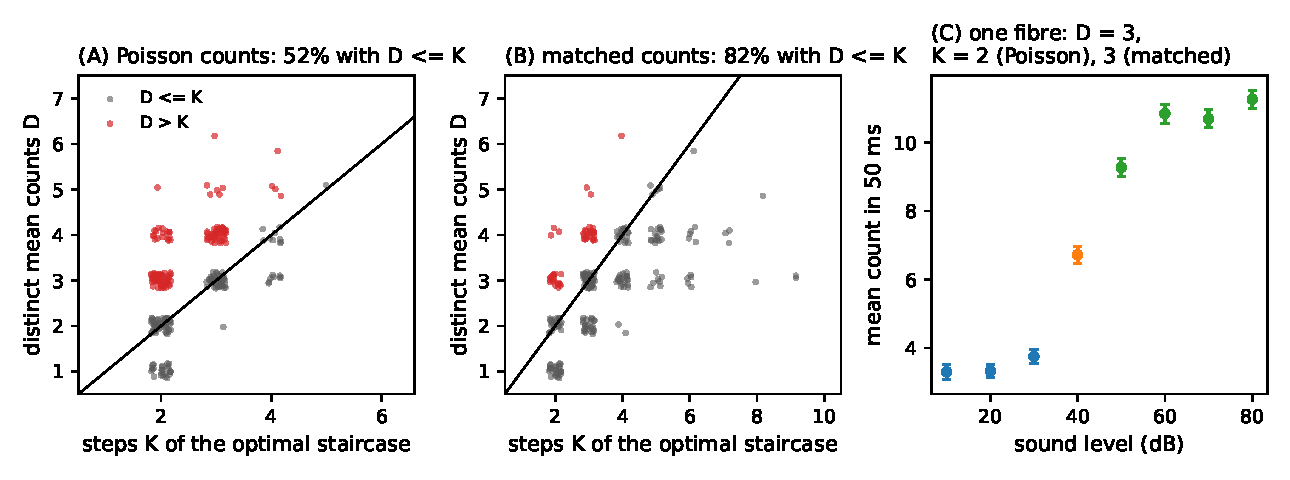
\includegraphics[width=\textwidth]{figs/fig_dk.pdf}
\caption{\textbf{Distinct mean counts against the steps of the optimal staircase.} (A) For each of the 265 fibres, the number $D$ of
significantly different mean counts against the number $K$ of steps computed for Poisson counts; points are shifted slightly so that
they do not overlap, and points on or below the line $D=K$ meet the bound. (B) The same with $K$ computed for counts matched to each
fibre's Fano factor; three fibres with $K$ above 10 are not shown, and all three meet the bound. (C) One fibre, chosen by a fixed rule
among the 59 fibres that meet the bound with the matched $K$ but not with the Poisson $K$: the one whose peak count is the median of
that set ($A=7.98$, spontaneous count $3.3$). Mean counts per sound level with standard errors; levels that the test does not separate
share a colour, so the three colours are its $D=3$ distinct mean counts.}\label{fig:dk}
\end{figure}

A larger $K$ is easier to meet, but a registered synthetic control with counts as regular as these shows that graded tuning curves
meet it in only $16.0\%$ and $0.5\%$ of cases at peak counts 8 and 15 (Section~\ref{sec:methods}). Among the 118 fibres with a peak
count of at least 8, where the test separates the two codes, the bound held in $92.4\%$ with the matched $K$ and in $83.9\%$ with
the $K$ matched at every rate; this split was computed after the tests. Below that peak count a graded fibre can meet the bound as well, so those 147 fibres carry little evidence either way.
Among them the bound held in $74.1\%$ with the matched $K$ and in $71.4\%$ with the $K$ matched at every rate, so they lower the fraction over all fibres and do not raise it.

Pooled over fibres, the auditory-nerve fibres thus favour the shape that Barlow's principle predicts for natural sound levels over a
symmetric sigmoid, in young and in aged animals. Under Poisson counts about half of them use more distinct rates than the staircase allows. Their
counts are far more regular than Poisson counts. With the staircase computed for a count matched to the mean regularity of each fibre,
more than four in five fibres are consistent with it, a bound that graded tuning curves of the same regularity rarely meet. With the
regularity matched at every rate, which fits the counts best, about three in four are, short of the registered $80\%$. Among the
fibres with a peak count of at least 8, where the test can tell a staircase from a graded curve, more than four in five are. The
likelihood test, which has more power than the count $D$, finds about half of the fibres consistent with the optimal number of
steps and nearly nine in ten consistent with one step more. The fibres use few rates, close to the optimal number; about half
need more steps than the optimum, most of them one more.
